\documentclass{beamer}
\usepackage{listings,amsmath,../../design/aux/proof}
\usepackage{pgf,pgfarrows,pgfnodes,tikz}

%%!TEX root = manual.tex
%
\chapter{ASDL Syntax}
\label{chap:syntax}

This section describes the syntax of the input language to \asdlgen{}.
The syntax is described using EBNF notation.
Literal terminals are typeset in \lit{bold} and enclosed in single quotes.
Optional terms are enclosed in square brackets and terms that are
repeated zero or more times are enclosed in braces.
Each section describes a fragment of the syntax and its meaning.

\section{Lexical Tokens}

The lexical conventions for \asdl{} are given in \figref{fig:lexical-syntax}.
ASDL is a case-sensitive language and, furthermore, classifies identifiers
into initial-lower-case (\synt{lc-id}) and initial-upper-case (\synt{uc-id}) identifiers.
Type identifiers are initial-lower-case, while constructor identifiers are initial-upper-case.
Module and field identifiers can be either upper or lower-case.

\begin{figure}[t]
  \begin{quote}
    \begin{grammar}
      <upper>     ::= `A' | ... | `Z'

      <lower>     ::= `a' | ... | `z'

      <alpha>     ::= `_' | <upper> | <lower>

      <alpha-num> ::= <alpha> | `0' | ... | `9'

      <lc-id>     ::= <lower> \{ <alpha-num> \}
      
      <uc-id>     ::= <upper> \{ <alpha-num> \}

      <id>        ::= <lc-id> | <uc-id>
                  
      <typ-id>    ::= <lc-id>

      <con-id>    ::= <uc-id>

      <comment>   ::= `--' \{ <text-character> \} <end-of-line>

      <text>      ::= `:' \{ <text-character> \} <end-of-line>
               \alt{} `\%\%' \{ <text-character> | <end-of-line> \} <end-of-line> `\%\%'
    \end{grammar}
  \end{quote}
  \caption{Lexical rules for \asdl{} terminals}
  \label{fig:lexical-syntax}
\end{figure}%

Comments begin with \lit{--}
and continue to the end of the line.

Verbatim text is denoted by \synt{text} and can be specified in one of two ways.
Either by an initial \lit{:} followed by a sequence of \synt{text-character}s that
continues to the end of the line or by a \lit{\%\%} terminated by a \lit{\%\%}
at the beginning of a line by itself. 
Text included using the `\lit{:} notation will have trailing and leading 
whitespace removed.

ASDL has the following keywords:
\begin{quote}
  \lit{alias}  \lit{attributes} \lit{import}
  \lit{include} \lit{module} \lit{primitive} \lit{view}
\end{quote}%
Note that it is allowed to use a keyword as an identifier wherever a \synt{lc-id} is permitted.

\section{File Syntax}

An \asdl{} file consists of one or more \synt{definition}s possibly preceded by \lit{include}
directives.
A definition specifies either a module (see \secref{sec:module-syntax}),
primitive module (see \secref{sec:primitive-syntax}),
or view (see \secref{sec:view-syntax}).

Include directives allow one to split a large \asdl{} specification into multiple files,
while allowing \asdlgen{} to check references from one module to another.
\asdlgen{} will parse included files, but will not generate code for the definitions in included
files.
Also, included files will only be parsed once.

\begin{figure}[t]
  \begin{quote}
    \begin{grammar}
      <file>  ::=  \{ `include' <text> \} <definition> \{ <definition> \}
      
      <definition> ::= <module>
        \alt{} <primitive-module>
        \alt{} <view>
    \end{grammar}
  \end{quote}
  \caption{\asdl{} file syntax}
  \label{fig:file-syntax}
\end{figure}%

\section{Module Syntax}
\label{sec:module-syntax}

\figref{fig:module-syntax} gives the syntax for modules.
An \asdl{} module declaration consists of the keyword \lit{module}
followed by an identifier, an optional set of imported modules, and a
sequence of type definitions enclosed in braces.

\begin{figure}[t]
  \begin{quote}
    \begin{grammar}
      <module>  ::=  `module' <id> [ <imports> ] `{' \{ <type-definition> \} `}'

      <imports> ::=  `(' \{ `import' <id> [ `alias' <id> ] \} `)'
    \end{grammar}
  \end{quote}
  \caption{\asdl{} module syntax}
  \label{fig:module-syntax}
\end{figure}%

For example the
following example declares modules \lstinline[language=ASDL]!A!,
\lstinline[language=ASDL]!B!, and \lstinline[language=ASDL]!C!.
\lstinline[language=ASDL]!B! imports types from \lstinline[language=ASDL]!A!.
\lstinline[language=ASDL]!C! imports types from both \lstinline[language=ASDL]!A! and
\lstinline[language=ASDL]!B!.
Imports cannot be recursive; for example, it is an error for \lstinline[language=ASDL]!B! to
import \lstinline[language=ASDL]!C!, since \lstinline[language=ASDL]!C!
imports \lstinline[language=ASDL]!B!.
\begin{code}\begin{lstlisting}[language=ASDL]
 module A { ... } 
 module B (import A) { ... }
 module C (import A 
           import B) { ... }
\end{lstlisting}\end{code}% 

To refer to a type imported from another module the type must
\emph{always} be qualified by the module name from which it is
imported.
The following declares two different types called ``\texttt{t}.''
One in module \texttt{A} and one in module \texttt{B}.
The type ``\texttt{t}'' in module \texttt{B} defines a type ``\texttt{t}'' that
recursively mentions itself and also references the type ``\texttt{t}'' imported
from module \texttt{A}.
\begin{code}\begin{lstlisting}[language=ASDL]
module A { t = ... } 
module B (import A) { t = T(A.t, t) | N  ... }
\end{lstlisting}\end{code}% 

\section{Type Definitions}

The syntax of type definitions is given in \figref{fig:type-syntax}.
A type defintion begins with a type identifier, which is the name of the type.
The name must be unique within the module, but the order of definitions is unimportant.
When translating type definitions from a module they are placed in what would be considered a
module, package, or name-space of the same name.
If the output language does not support such features and only has one global
name space the module name
is used to prefix all the globally exported identifiers.

\begin{figure}[t]
  \begin{quote}
    \begin{grammar}
      <type-definition>  ::=  <typ-id> `=' <type>

      <type>         ::= <alias-type> | <sum-type> | <product-type>

      <alias-type>   ::= <typ-exp>
      
      <product-type> ::= <fields>

      <sum-type>     ::= <constructor> \{ `|' <constructor> \} [ `attributes' <fields> ]

      <constructor>  ::= <con-id> [ <fields> ]

      <fields>       ::= `(' \{ <field>  `,' \} <field> `)'

      <field>        ::=  <typ-exp> [ <id> ]
      
      <typ-exp>      ::= [ <id> `.' ] <typ-id> [ `?' | `*' | `!' ]
    \end{grammar}
  \end{quote}
  \caption{\asdl{} type definition syntax}
  \label{fig:type-syntax}
\end{figure}%

Type definitions are either alias types, which bind a name to a type expression;
product types, which are simple record definitions;
or sum type, which represent a discriminated union of possible values.
Unlike sum types, product types cannot form recursive type definitions, but they can
contain recursively declared sum types.

\subsection{Alias Types}

Alias types are the simplest form of type definition.
They provide a way to give a name to a type or type expression, similar
to \sml{}'s \lstinline[language=SML]@type@ and \Cplusplus{}'s
\lstinline[language=C++]@typedef@ constructs.

\subsection{Type expressions}

A type expression (\synt{typ-exp}) consists of a possibly qualified type name followed
by an optional type operator.
If the specified type is an ASDL primitive type or is defined in the current module,
then its name is not qualified; all other types defined outside the current module must
be qualified by their module name (or module alias).

The type operators are:
\begin{itemize}
  \item
    option (\lit{?}), which specifies either zero or one value of the specified type.
  \item
    sequence (\lit{*}), which specifies a sequence of zero or more values of the
    specified type, or
  \item
    shared (\lit{!}), which specifies that a value is shared across multiple points
    in the data structure (\ie{}, the structure has a DAG shape instead of just a tree).
\end{itemize}%

Note that while at most one type operator is allowed in a type expression, one can use alias
types to combine two or more operators.
For example, a sequence of optional integers could be defined by:
\begin{code}\begin{lstlisting}[language=ASDL]
int_opt = integer?
int_opt_seq = int_opt*
\end{lstlisting}\end{code}%

\subsection{ASDL Primitive Types}
There are seven pre-defined primitive types in ASDL, which are available without qualification:
\begin{description}
  \item[\normalfont\texttt{\color{\cdColor}bool}] describes Boolean values.
  \item[\normalfont\texttt{\color{\cdColor}int}] describes signed-integer values that are representable in 30 bits
    (\ie{}, in the range ${-}2^{29}$ to~\mbox{$2^{29}-1$}).
  \item[\normalfont\texttt{\color{\cdColor}uint}] describes unsigned-integer values that representable in 30 bits
    (\ie{}, in the range $0$ to~$2^{30}-1$).
  \item[\normalfont\texttt{\color{\cdColor}integer}] describes arbitrary-precision signed-integer values.
  \item[\normalfont\texttt{\color{\cdColor}natural}] describes arbitrary-precision unsigned-integer values.
  \item[\normalfont\texttt{\color{\cdColor}string}] describes length encoded strings of 8-bit characters.
  \item[\normalfont\texttt{\color{\cdColor}identifier}] describes strings with fast equality testing
    analogous to Lisp symbols.
\end{description}%

% TODO: Not implemented yet
%In addition, the \lstinline!StdTypes! module defines additional fixed-precision numeric types
%that can be used when necessary (\eg{}, \lstinline!StdTypes.int32!).

\subsection{Product Types}
Product types are defined by a non-empty  sequence of fields separated by
commas enclosed in parenthesis.
A field consists of a type expression followed by an optional label.
The fields of a product or sum type must either all be labeled or unlabeled.
We use \emph{record} to refer to products of labeled fields and \emph{tuple}
to products of unlabeled fields.
Labels aid in the readability of
descriptions and are used by \asdlgen{} to name the fields of records
and classes for languages.

For example, the declaration
\begin{code}\begin{lstlisting}[language=ASDL] 
pair_of_ints = (int, int) 
\end{lstlisting}\end{code}% 
defines the tuple type \lstinline[language=ASDL]!pair_of_ints! that consists of two integers,
whereas the declaration
\begin{code}\begin{lstlisting}[language=ASDL] 
size = (int width, int height) 
\end{lstlisting}\end{code}%
defines the record type \lstinline[language=ASDL]!size! that consists of two
labeled fields: \lstinline[language=ASDL]@width@ and \lstinline[language=ASDL]@height@.
Note that ASDL requires that if any field in a product type has a label, then all
of them must have labels.

For the \sml{} target, product types without labels are translated to tuples, while
those with labels are translated to records.

\subsection{Sum Types}

Sum types are the most useful types in ASDL. They provide concise notation
used to describe a type that is the tagged union of a finite set of other
types.  Sum types consists of a series of constructors separated by a
vertical bar. Each constructor consist of a constructor identifier followed
by an optional product type. 

Constructor names must be unique within the module in which they are
declared. Constructors can be viewed as functions who take some number of
arguments of arbitrary type and create a value belonging to the sum type in
which they are declared.
For example
\begin{code}\begin{lstlisting}[language=ASDL]
module M {
  sexpr = Int(int)
	| String(string)
	| Symbol(identifier)
	| Cons(sexpr, sexpr)
	| Nil
}
\end{lstlisting}\end{code}%
declares that values of type \lstinline[language=ASDL]!sexpr! can either be
constructed from an \lstinline[language=ASDL]!int! using the
\lstinline[language=ASDL]!Int! constructor or a \lstinline[language=ASDL]!string!
from a \lstinline[language=ASDL]!String! constructor, an
\lstinline[language=ASDL]!identifier! using the \lstinline[language=ASDL]!Symbol!
constructor, from two other \lstinline[language=ASDL]!sexpr! using the
\lstinline[language=ASDL]!Cons! constructor, or from no arguments
using the \lstinline[language=ASDL]!Nil! constructor.
Notice that the \lstinline[language=ASDL]!Cons! constructor
recursively refers to the \lstinline[language=ASDL]!sexpr! type.
\asdl{} allows sum types to be mutually recursive.
Recursion, however, is limited to sum types defined within the same module.

\subsubsection{Sum Types as Enumerations}
\label{sec:enumerations}

Sum types that consist completely of nullary constructors
are often treated specially and translated into static constants of a
enumerated value in languages that support them.
For example, the following \asdl{} specification:
%
\begin{code}\begin{lstlisting}[language=ASDL]
module Op {
  op = PLUS | MINUS | TIMES | DIVIDE 
}
\end{lstlisting}\end{code}%
%
Is translated into the following \Cplusplus{} code:
%
\begin{code}\begin{lstlisting}[language=c++]
namespace M {
    enum class op {
        PLUS = 1, MINUS, TIMES, DIVIDE
    };
}
\end{lstlisting}\end{code}%

\subsubsection{Attribute Fields}
A sum-type definition may optionally be followed by a list of attribute fields, which
provide a concise way to specify fields that are common to all of the constructors
of a sum type.
For example, the definition
%
\begin{code}\begin{lstlisting}[language=ASDL]
module M {
  pos = (string file, int linenum, int charpos)
  sexpr = Int(int)
	| String(string)
	| Symbol(identifier)
	| Cons(sexpr, sexpr)
	| Nil
        attribute(pos)
}
\end{lstlisting}\end{code}%
adds a field of type \lstinline[language=ASDL]!pos! to all the constructors
in \lstinline[language=ASDL]!sexpr!.
One can think of an \lstinline!attribute! annotation as syntactic sugar for just including
the extra fields at the \emph{beginning} of each constructor's fields.
For example, the above definition can be viewed as syntactic sugar for
%
\begin{code}\begin{lstlisting}[language=ASDL]
module M {
  pos = (string file, int linenum, int charpos)
  sexpr = Int(pos, int)
	| String(pos, string)
	| Symbol(pos, identifier)
	| Cons(pos, sexpr, sexpr)
	| Nil(pos)
}
\end{lstlisting}\end{code}%
Note that this interpretation implies that attribute fields are labeled if, and only if, all
of the constructor fields are labeled.

Attribute fields are treated specially when translating to some targets.
For example in \Cplusplus{} code, the attribute field is defined in the base class for the sum type.

\section{Primitive Modules}
\label{sec:primitive-syntax}

\begin{figure}[t]
  \begin{quote}
    \begin{grammar}
      <primitive-module> ::= `primitive' `module' <id> `{' \{ <id> \} `}'
    \end{grammar}%
  \end{quote}%
  \caption{\asdl{} primitive module syntax}
  \label{fig:prim-module-syntax}
\end{figure}%

Primitive modules (see \figref{fig:prim-module-syntax}) provide a way to introduce abstract
types that are defined outside
of \asdl{} and which have their own pickling and unpickling code.
For example, we might want to include GUIDs (16-byte globally-unique IDs) in our pickles.
We can do so by first defining a primitive module \lstinline!Prim!:
%
\begin{quote}\begin{lstlisting}[language=ASDL]
primitive module Prim { guid }
\end{lstlisting}\end{quote}%
%
Then, depending on the target language, we define
supporting code to read and write guids from the byte stream.
In \sml{}, we would define two modules:
\begin{enumerate}
  \item \lstinline[language=SML]!structure Prim! that defines the representation of the
    \lstinline[language=SML]!guid! type.
  \item
    \lstinline[language=SML]!structure PrimPickle! that defines functions
    for pickling/unpickling a GUID using an imperative stream API.
\end{enumerate}%
The \sml{} implementation of these modules could be written as follows:
\begin{code}\begin{lstlisting}[language=SML]
structure Prim : sig
    type guid
  end = struct
    type guid = GUID.guid
  end

structure PrimPickle : sig

    val read_guid : (unit -> Word8.word) -> unit -> Prim.guid
    val write_guid : (Word8.word -> unit) -> Prim.guid -> unit
    
  end = struct
  
    val guidSize = 16
    fun read_guid getByte () =
          GUID.fromBytes(Word8Vector.tabulate(guidSize, fn _ => getByte()))
    fun write_guid putByte guid = let
          Word8Vector.app putByte (GUID.toBytes guid)

   end
\end{lstlisting}\end{code}%
(assuming that the \lstinline!GUID! module implements the application's representation
of GUIDs).

For \Cplusplus{}, a primitive module requires a corresponding header file that declares
the primitive types and instances of the overloaded \lstinline[language=c++]!<<! and
\lstinline[language=c++]!>>! operators on the primitive types.  These declarations should
all be in a \lstinline[language=c++]!namespace! with the type name of the primitive module.
For example, the module from above would require the provision of a \texttt{Prim.hxx} header
file that contained something like the following code:
%
\begin{code}\begin{lstlisting}[language=c++]
#include <iostream>
#include "guid.hxx"

namespace Prim {

    typedef GUID::guid guid;

    std::istream &operator>> (std::istream &is, guid &g);
    std::ostream &operator<< (std::ostream &os, guid const &g);

}
\end{lstlisting}\end{code}%
(assuming that the \texttt{guid.hxx} header defines the application's representation
of GUIDs).
%For the \Cplusplus{} target, one should use string streams (in binary mode)
%to support pickling/unpickling of to/from memory.


\section{View Syntax}
\label{sec:view-syntax}

A view defines how an \asdl{} specification is translated to a target.
Each of the supported targets (\eg{}, \sml{} or \Cplusplus{}) has a default
view, but it is possible to customize the translation using \synt{view}
definitions.
The syntax of view declarations is given in \figref{fig:view-syntax}.
This section covers the syntax of views, but leaves the semantics to
\chapref{chap:views}.

\begin{figure}[t]
  \begin{quote}
    \begin{grammar}
      <view>        ::= `view' <id> `{' \{ <view-entry> \} `}'

      <view-entry>  ::=  <view-entities> `<=' <view-properties>
         \alt{} `<=' <id> `{' \{ <view-entity> <text> \} `}'

      <view-entities> ::= <view-entity>
         \alt{} `{' \{ <view-entity> \} `}'

      <view-entity> ::= `<file>'
         \alt{} `module' <id>
         \alt{} <id> `.' <typ-id> [ `.' `*' ]
         \alt{} <id> `.' <typ-id> `.' <con-id>

      <view-properties> ::= <id> <text>
          \alt{} `{' \{ <id> <text> \} `}'
    \end{grammar}%
  \end{quote}%
  \caption{\asdl{} view syntax}
  \label{fig:view-syntax}
\end{figure}%

\subsection{Basic View Syntax}
Views are named and consist of series of entries.
In its basic form, a view entry consists of a \synt{view-entity}, which specifies a file, module,
type, or constructor entity, and a view property, which is a name-value pair that is associated with
the entity.
%
\begin{quote}\begin{grammar}
  <view-entry>  ::= <view-entity> `<=' <id> <text>
\end{grammar}\end{quote}%
%
The meaning of an entry is to associate the specified view property with the specified view entity.
%%
%\begin{code}\begin{lstlisting}[language=ASDL]
%view Doc {
%  module  M <= doc_string
%%%
%  Types for representing LISP s-expressions.
%%%
%  M.sexpr  <= doc_string : s-expressions 
%  M.Int    <= doc_string : s-expression constructor
%  M.Symbol <= doc_string : s-expression constructor
%  M.Cons   <= doc_string : s-expression constructor
%  M.Nil    <= doc_string : s-expression constructor
%}
%
%view Java {
% M.sexpr <= source_name : Sexpr
% M.sexpr <= base_class  : MyClass
%}
%\end{lstlisting}\end{code}%
%%
%associates with the module \lstinline[language=ASDL]!M! the type
%\lstinline[language=ASDL]!M.sexpr! and the
%constructor \lstinline[language=ASDL]!M.Int!
%strings that will be added to the automatically generated documentation
%produced by the \texttt{--doc} command of \asdlgen{}.
%(\emph{In future we will probably dump them in comments in the output code too.})
%The view named \lstinline[language=ASDL]!Java! causes the type
%\lstinline[language=ASDL]!M.sexpr! to be renamed \lstinline[language=ASDL]!Sexpr! when
%generating Java output, and causes the abstract class normally generated to
%inherit from \lstinline[language=ASDL]!MyClass!. 

There can be multiple views with the same name.
The entries of two views with the same name are merged and consist of the
union of the entries in both.
It is an error, for two views of the same name to assign different values
to the same property of an entity.

\subsection{View Entry Derived Forms}
To make it easier to specify view entries, \asdl{} generalizes the basic syntax
to remove some of the redundancy of the basic syntax.
First, it is possible to specify multiple view entities on the left-hand-side of
the \lit{<=} symbol.
Likewise, it is possible to specify multiple view properties on the right-hand-side
of the \lit{<=} symbol.

It is also possible to assign different values to different entities for a fixed property
using the syntax.
%
\begin{quote}\begin{grammar}
  <view-entry> ::= `<=' <id> `{' \{ <view-entity> <text> \} `}'
\end{grammar}\end{quote}%
%
Here the property name is given first, followed by a sequence of view-entity-value pairs.

Lastly, \asdl{} allows a \lit{.*} suffix to be added to sum-type entities.
This suffix means that the entity specifies the set of all of the constructors of the type.

%Examples of the sugared notation are shown
%below in their respective order.
%\begin{code}\begin{lstlisting}[language=ASDL]
%view Doc {
% { M.Int  M.Symbol  
%   M.Cons M.Nil } <= doc_string : s-expression constructor
%
% <= doc_string {
%  module  M 
%%%
%  Types for representing LISP s-expressions.
%%%
%  M.sexpr : s-expressions 
%  }
%}
%
%view Cxx {
%  M.sexpr <= {
%    source_name : Sexpr
%    base_class  : MyClass
%  }
%}
%\end{lstlisting}\end{code}%


\newcommand{\letx}{\ensuremath{\mathsf{let}}}
\newcommand{\lettycline}[2]{\ensuremath{\begin{array}{l}
\mathsf{let~tyc}~#1\\\mathsf{in}~#2\end{array}}}
\newcommand{\tyc}{\ensuremath{\mathsf{tyc}}}
\newcommand{\inx}{\ensuremath{\mathsf{in}}}
\newcommand{\inlet}{\ensuremath{\mathsf{in~let}}}
\newcommand{\letin}[2]{\ensuremath{\mathsf{let}~#1~\mathsf{in}~#2}}
\newcommand{\newx}{\ensuremath{\mathsf{new}}}
\newcommand{\chk}{\ding{51}}
\newcommand{\ex}{\ding{55}}

\lstset{escapeinside=`',columns=fullflexible}
\setbeamercovered{invisible}
\usetheme{Luebeck}
%\usecolortheme{seagull}
%\useinnertheme{rectangles}
%\useoutertheme{infolines}

\mode<presentation>
\setbeamertemplate{navigation symbols}{}

\lstset{language=ML,basicstyle=\small}

\tikzstyle{every picture}+=[remember picture]
\everymath{\displaystyle}
\tikzstyle{na} = [baseline=-.5ex]
\tikzstyle{arr} = [line width=2pt,->]
\tikzstyle{block} = [rectangle, draw, fill=blue!20, 
    text width=5em, text centered, rounded corners, minimum height=4em]


\title[A True Higher-Order Module System]{A True Higher-Order Module System}
\author{George Kuan}
%\institute{University of Chicago}
\date{Dissertation Defense\\ May 3, 2010}

\begin{document}
	
	\begin{frame}
		\maketitle
	\end{frame}

	\begin{frame}[fragile]
		\frametitle{Higher-Order Modules}
		\begin{itemize}[<+->] 
			\item[]
		\begin{lstlisting}
		signature T = sig type t end
		functor Apply(functor F(X:T):T) (M:T) = F(M)
		\end{lstlisting}
			\item[]
		\begin{lstlisting}
		functor Id(X:sig type t end) = X
		structure N = Apply (functor F=Id) (struct type t = int end)
		\end{lstlisting}
			\item[] \alert<.>{Expect N.t = int}
			\item[]
		\begin{lstlisting}
		functor Const(X:sig type t end) = struct type t = bool end
		structure R = Apply (functor F=Const) (struct type t = int end)
		\end{lstlisting}
			\item[] \alert<.>{Expect R.t = bool}
		\end{itemize}
	\end{frame}
	
	% \begin{frame}[fragile]
	% 	\frametitle{True Higher-Order Semantics (2)}
	% 	\begin{itemize}[<+->]
	% 	\item[]
	% 	\begin{lstlisting}
	% 	functor F() = 
	% 	struct 
	% 	  datatype t = S of int 
	% 	  val m = S 0 
	% 	end	
	% 	\end{lstlisting}
	% 	
	% 	\item[]
	% 	\begin{lstlisting}
	% 	structure M0 = F()
	% 	\end{lstlisting}
	% 	
	% 	\item[]
	% 	\begin{lstlisting}
	% 	structure M1 = F()
	% 	\end{lstlisting}
	% 	
	% 	\item[] \alert{M0.t $\ne$ M1.t}
	% 	\end{itemize}
	% \end{frame}

		\begin{frame}[fragile]
			\frametitle{Approaches (1)}
			\begin{enumerate}[<+->]
				\item Syntactic (Applicative Functors [Leroy 1995])~\\

	functor Apply(functor F(X:T):T) (M:T) \\
	  : sig type t=\tikz[baseline]{\node[fill=blue!20,anchor=base](t1){F(M).t}} end = F(M) 	

				\item[] \hspace{10em}\tikz[na] \node[coordinate] (n1) {}; \alert<.>{can only be treated superficially} 
				\item Semantic [MacQueen-Tofte 1994]~\\

	functor Apply(functor F(X:T):T) (M:T) \\
	~~: sig type t end = F(M) 	\\[3mm]


	Dependence of result type t on F and M is inferred by the compiler

			\end{enumerate}

			\begin{tikzpicture}[overlay]
				\path[->]<2-> (n1) edge [bend left] (t1);
			\end{tikzpicture}
		\end{frame}



		\begin{frame}[fragile]
			\frametitle{Approaches (2)}
			\begin{lstlisting}
			functor F(functor G(X:T):T) = 
			struct 
			  datatype s = S of int 
			  structure M = G(struct type t = s end)
			  type u = M.t
			end	
			\end{lstlisting}

			\uncover<2->{Syntactic approach breaks down.}\\
			\only<3->{A descriptive signature would have to involve static effects and the  actions taken by formal functor G.}

		\end{frame}
			
	\begin{frame}
		\frametitle{True Higher-Order Semantics }
		\begin{block}{Functor Action}
		A \alert{function action} is the way in which a functor computes its output types from its parameter types, namely: 
		\begin{enumerate} 
			\item type generativity 
			\item functor actions of formal functors
		\end{enumerate}
		\end{block}
	\end{frame}
	
	\begin{frame}
		\frametitle{Motivation}
		\begin{block}{Syntactic Approaches}
			All module type information is syntactic
			\begin{enumerate}
				\item Give up non-syntactic module type information
				\item Try to express more module type information syntactically 
			\end{enumerate}
		\end{block}
		\vspace{4mm}
		\begin{block}{Semantic Approach}
			Some module type information is semantic (functor actions)
		\end{block}
	\end{frame}
	
	\begin{frame}[fragile]
		\frametitle{Motivation}
		\begin{enumerate}
			\itemsep=4mm
			\item Restricting to syntactic module types is analogous to restricting a language to $\lambda$-terms where each $\lambda$ is given a really powerful dependent type that computes the result of the $\lambda$
			\item An abstract model of current SML/NJ implementation of higher-order modules
			\item A more detailed and realistic expansion of MacQueen-Tofte~1994 and  Shao~1998 
			\item True higher-order semantics without re-elaboration
		\end{enumerate}
	\end{frame}
		
	\begin{frame}
		\frametitle{Outline}
		\tableofcontents
	\end{frame}
	
	\section{Type of a Structure}

\begin{frame}
	\frametitle{Type of a Structure}
	{\Large Big Question: What is the ``type'' of a structure?}
\end{frame}

\begin{frame}
	\frametitle{Signatures}
structure A = struct\\
~~datatype $\alpha$ t = c of $\alpha$\\
~~structure M = struct datatype t = d val x = c d end\\
end\\[2mm]

\only<1>{Syntactic}\only<2->{{\color{blue}Semantic}} Signature\\[1mm]
sig\\
~~type $\alpha$ t \tikz[na] \node[coordinate] (n0) {};\uncover<2->{{\color{blue}$\rho_0$}}\\
~~structure M \uncover<2->{{\color{blue}$\rho_M$}}: sig~type~ t~\uncover<2->{{\color{blue}$\rho_1$}}~val~x: \only<1>{\tikz[na] \node[coordinate,yshift=3mm] (t0) {};\alert{??}} \only<2->{{\color{blue}\tikz[baseline]{\node[anchor=base](t1) {$\rho_0(\rho_1)$};}}}
%~val~k : \only<1>{$(\alpha, $ t}\only<2->{{\color{blue}\tikz[baseline]{\node[anchor=base] (t2) {$\forall\alpha.\rho_1(\alpha,\rho_0)$}; }}} 
end\\
end\\[3mm]
\only<2>{Because type names can shadow, syntactic names are insufficient}
\only<3>{Need unshadowable \alert{entity variables} (\emph{aka} internal names  [Harper-Lillibridge 94]) and \alert{entity paths} (\emph{e.g.}, $\rho_M\rho_1$)}
\only<4>{\hspace{8em}\tikz{\node (s0) {relativized types};}}
\uncover<5->{
Abbreviated: 
\[\left\{\begin{array}{l}
t : (\rho_0, 1),\\
M : (\rho_M, \{t : (\rho_1, 0),~x : \rho_0(\rho_1) \})\\
\end{array}
\right\}
\]}
\begin{tikzpicture}[overlay]
	\path[arr]<1> (n0) edge [bend left] (t0);
	
	\path[arr]<4> (s0) edge [bend right] (t1);
	%\path[arr]<4> (s0) edge [bend right] (t2);
\end{tikzpicture}

\end{frame}

\begin{frame}
	\frametitle{Type of a Structure}
	functor F() = struct\\
	~~structure M = struct datatype~t end\\
	~~val x : M.t = ...\\
	end\\
	\vspace{1em}
	structure A = F()\\[2em]

	\only<1-2>{What is the module ``type'' for A?}
	\uncover<2->{
	$\left\{\begin{array}{l}
	M:(\rho_M, \{t : (\rho_t, 0)\}),~x : \rho_M\rho_t
	\end{array}
	\right\}
	$\\[1em]}

	\only<+>{A semantic signature is not the complete module ``type''.}
	\uncover<+>{Need an \alert{entity environment} mapping entity variables to static entities (tycons, structures, and functors) $\{ \rho_M\mapsto\{\rho_t\mapsto \tau^0\} \}$\\ $\tau^0$ is a fresh atomic semantic tycon}

\end{frame}

\begin{frame}
	\frametitle{Entity Environments}
	functor F() = struct\\
	~~structure M = struct datatype~t end\\
	~~val x : M.t = ...\\
	end\\[1em]
\begin{itemize}[<+->]
	\item[] structure A = F() \hspace{4em} $\rho_A \mapsto \{ \rho_M\mapsto\{\rho_t\mapsto \tau^{0}_a\} \}$
	\item[] structure B = F() \hspace{4em} $\rho_B \mapsto \{ \rho_M\mapsto\{\rho_t\mapsto \tau^0_b\} \}$
\end{itemize}
\uncover<2>{Each time F is applied, we get 
 a fresh atomic tycon}	
\end{frame}

\begin{frame}
	\frametitle{Full Signature}
	\begin{equation*}
		\tikz[baseline]{\node[fill=blue!20,anchor=base] (n0) {$\left\{\begin{array}{l}
	M:(\rho_M, \{t : (\rho_t, 0)\}),~x : \rho_M\rho_t
	\end{array}
	\right\}$};}
	+ \tikz[baseline]{\node[fill=red!20,anchor=base] (n1) {$\{ \rho_M\mapsto\{\rho_t\mapsto \tau^0\} \}$};}
	\end{equation*}
	
	\begin{tikzpicture}[overlay]
		\node[above of=n0] (t0) {signature (fixed)};
		\node[above of=n1] {realization (volatile)};
	\end{tikzpicture}

\vspace{3em}
\uncover<2->{
	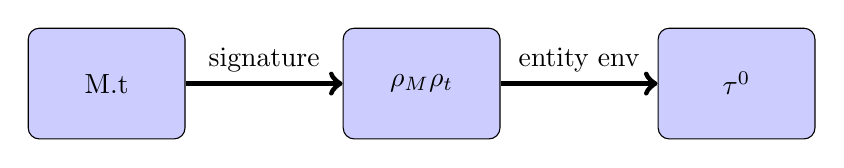
\begin{tikzpicture}[node distance=4cm, auto]
		\node[block] (n2) {M.t};
		\node[block, right of=n2] (n3) {$\rho_M\rho_t$};
		\node[block, right of=n3] (n4) {$\tau^0$};
		
		\path[arr] (n2) edge node {signature} (n3);
		\path[arr] (n3) edge node {entity env} (n4);
	\end{tikzpicture}}
	
	
\end{frame}

\begin{frame}
	\frametitle{Type of a Structure}
	{\Large But what is a functor entity?}
% \begin{itemize}[<+->]
% 	\item[] 
% 	\item[] An entity function $\lambda\rho.\varphi$ such that $\varphi$ is a structure entity expression that evaluates to a structure entity (realization)
% \end{itemize}

\uncover<2>{
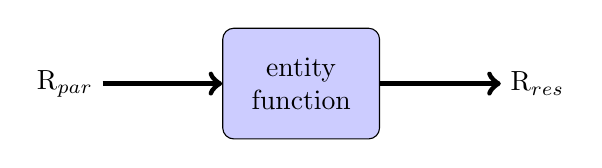
\begin{tikzpicture}[auto,node distance=3cm]
	\node (par) {R$_{par}$};
	\node[block,right of=par] (lam) {entity function};
	\node[right of=lam] (res) {R$_{res}$};
	
	\path[arr] (par) edge (lam);
	\path[arr] (lam) edge (res); 
	
\end{tikzpicture}}
\end{frame}

\section{Entity Calculus}

% \begin{frame}
% 	\frametitle{Entity Calculus}
% 	\begin{enumerate}
% 		\item Entity variable ($\rho$): unshadowable variable for static content (tycons, structures, and functors)
% 		\item Entity path ($\rho_0\rho_1\rho_2$): path into structure hierarchy 
% 		\item Entity environment: a finite map from entity variables to tycon, structure, and functor entities
% 	\end{enumerate}
% \end{frame}

\begin{frame}
	\frametitle{Entity Calculus (1)}
{\only<3>{\color{red}}datatype v}\\
functor F(X:sig type t end) = struct\\
~~{\only<2->{\color{blue}}datatype $(\alpha,\beta)$ u}\\
~~{\only<2,4>{\color{red}}type s = (X.t,v) u}\\
end\\[2em]
	\only<2>{A {\bf tycon entity} is either 
	\begin{itemize}
		\item an atomic tycon (\emph{e.g.}, {\only<2>{\color{blue}}$\tau^2_u$})
		\item or normal form semantic tycon (\emph{e.g.}, {\only<2>{\color{red}}$\lambda().\tau^2_u(\tau^0_t,\tau^0_v)$})
	\end{itemize}}
	\only<3>{A {\bf structure entity} $R$ is a pair of entity environments $\langle\{{\color{blue}\rho_u\mapsto\tau^2_u,~\rho_s\mapsto\lambda().\tau^2_u(\tau^0_t,\tau^0_v)}\},~~\{{\color{red}\rho_v\mapsto\tau^0_v}\}\rangle$\\[2mm]
	a local one defining all entities in the structure and a closure environment \\[2mm]
	$\tau^0_t$ is a dummy atomic tycon to stand in for the tycon in the functor argument }
	\uncover<4>{A {\bf functor entity} is a closure: a $\lambda$-expression mapping structure entity to an expression that evaluates to a structure entity $\lambda\rho_x.\{{\color{blue}\rho_u = \newx(2)}, {\color{red}\rho_s = \lambda().\rho_u(\rho_x\rho_t,\rho_v)} \}$ + $\{\rho_v\mapsto \tau^0_v\}$}
\end{frame}

\begin{frame}
	\frametitle{Entity Calculus (2)}
	\begin{itemize}
		\item[] Tycon entity expression:
		\[\zeta ::= \newx(n)~|~\mathbb{C}^\lambda \textrm{(relativized tycons)}\]
		\item[] Structure entity expression:
		\[ \varphi ::= \vec{\rho}~|~\{ \eta \}~|~\theta(\varphi)~|~ \letin{\eta}{\varphi}\]
		
		\item[] Functor entity expression:
		\[ \theta ::= \vec{\rho}~|~\lambda\rho.\varphi~|~\lambda\rho.\Sigma \]
		
		\item[] Entity declaration:
		\[ \eta ::= \circ~|~\rho = \zeta,\eta~|~\rho = \varphi,\eta~|~\rho = \theta,\eta\]
		
	\end{itemize}
\end{frame}

\begin{frame}
\frametitle{Life-Cycle of a Type}

\begin{tikzpicture}[node distance= 4.5cm,auto]
	\uncover<1->{\node[block] (sy) {Syntactic};}
	\uncover<2->{\node[block, right of=sy] (se) {Semantic};}
	\uncover<3->{\node[block, right of=se] (re) {Relativized};}

	\uncover<2->{\node[node distance=2cm,below of=se] (statenv) {static env};}
	\uncover<3->{\node[node distance=1cm,,below of=statenv] {entity env};}
	\uncover<3->{\node[node distance=2cm,below of=re] (semsig) {semantic sig};}
	\uncover<3->{\node[node distance=1cm,below of=semsig]  {entity expr};}
		
	\uncover<2->{\path[arr] (sy) edge node {\only<2>{\color{red}}elaborates} (se);}
	\uncover<3->{\path[arr] ([yshift=-5mm]se.north east) edge node {\only<3>{\color{red}}relativizes} ([yshift=-5mm]re.north west);}
	\uncover<3->{\path[arr] (se) edge [loop above] node {\only<3,4>{\color{red}}evaluates} (se);}
	\uncover<4->{\path[arr] ([yshift=5mm]re.south west) edge node {\only<4>{\color{red}}instantiates} ([yshift=5mm]se.south east);}
	

\end{tikzpicture}
\end{frame}

\begin{frame}[fragile]
	\frametitle{Functor Actions}
	\begin{itemize}[<+->]
		\item[]
	\begin{lstlisting}
	functor Apply(X:sig functor F(Y:sig type t end):sig type t end
	                    structure M: sig type t end
	                end) =
	struct structure R = X.F(X.M) end
	\end{lstlisting}
	\item[]
	\[\lambda\rho_x.\{\rho_r=\rho_x\rho_f(\rho_x\rho_m)\}\]
		\item[]
	\begin{lstlisting}
	functor G() = struct datatype t end	
	\end{lstlisting}
	\item[]
	\[\lambda().\{\rho_t=new(0)\}\]
	\end{itemize}
\end{frame}

\begin{frame}[fragile]
	\frametitle{Full Functor Signature}
	\begin{lstlisting}
	datatype v 
	functor F() = struct datatype t val a : v end	
	\end{lstlisting}
	
	\tikz[baseline]{\node[fill=blue!20,anchor=base] (sem) {Semantic functor signature};} + \tikz[baseline]{\node[fill=red!20,anchor=base] (ent) {Entity function (closure)};}
	
	\begin{tikzpicture}
	\node[below of=sem] {$\Pi().
	\{t : (\rho_t, 0),~a : \rho_v \}$};
	\node[below of=ent] {$\langle\lambda().\{\rho_t = \newx(0)\},~\{\rho_v\mapsto \tau^0\}\rangle$};
	\end{tikzpicture}
\end{frame}

\begin{frame}
	\frametitle{Constructing Full Signatures and Entity Expressions}
	Full signatures and entity expressions are produced by \alert{elaboration} in two interweaving modes:
	
	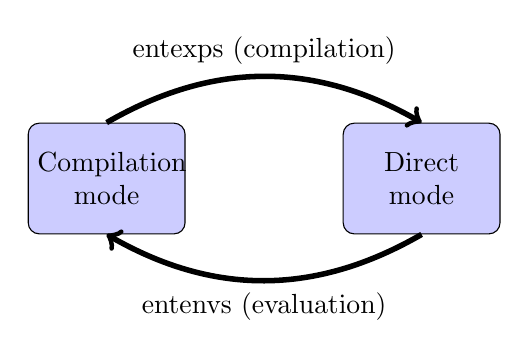
\begin{tikzpicture}[auto, node distance=4cm]
		\node[block] (cc) {Compilation mode};
		\node[block,right of=cc] (dm) {Direct mode};
		
		\path[arr] (cc.north) edge [bend left] node {entexps (compilation)} (dm.north);
		\path[arr] (dm.south) edge [bend left] node {entenvs (evaluation)} (cc.south);
	\end{tikzpicture}

\end{frame}

	% \begin{frame}[fragile]
	% 	\frametitle{Type System}
	% 
	% 	functor Symbols(functor F(X:T):T) = \\
	% 	struct \\
	% 	~~~datatype t = S of \tikz[baseline]{\node[fill=red!20,anchor=base](t0){int}} \\
	% 	~~~structure M = F(struct type t= \tikz[baseline]{\node[fill=red!20,anchor=base](t2){t}} end)\\
	% 	~~~type u = \tikz[baseline]{\node[fill=red!20,anchor=base](t3){M.t * bool}}\\
	% 	end	\\
	% 
	% 	\begin{enumerate}[<+->]
	% 		\item Syntactic types \tikz[na] \node[coordinate] (n0) {}; 
	% 		\item[] \hspace{15em} \tikz[na] \node[coordinate] (n1) {}; symbolic paths			 
	% 		\item Semantic types
	% 		\begin{enumerate}
	% 			\item no paths: symbolic paths looked up
	% 			\item generated datatypes and opaque tycons manifested (represented as $\tau^n$ where $n$ is arity) 
	% 			\item can be evaluated (by $\beta$-reduction) to a normal form
	% 		\end{enumerate}
	% 		\item Relativized
	% 	\end{enumerate}
	% 	
	% 	\begin{tikzpicture}[overlay]
	% 		\path[->]<1-> (n0) edge [bend right] (t0);
	% 		\path[->]<1-> (n0) edge [bend right] (t2);
	% 		\path[->]<1-> (n0) edge [bend right] (t3);
	% 		\path[->]<2-> (n1) edge [bend left] (t3.south west);
	% 	\end{tikzpicture}
	% \end{frame}
	

	\section{Elaboration}
	
	\begin{frame}
		\frametitle{Structure Elaboration}
		$\Gamma,\Upsilon\vdash strexp \Rightarrow_{str} (M, \varphi)$
		
		\begin{enumerate}[<+->]
			\item $\Gamma$ is the static environment mapping symbols to semantic tycons, full signatures, full functor signatures 
			\item $\Upsilon$ is the entity environment
			\item Full signature $M=\langle \Sigma, R\rangle$ where $\Sigma$ is the semantic signature and $R$ is the structure entity
			\item Structure entity expression $\varphi$: Evaluates to an $R'$ isomorphic to $R$ under the current entity environment $\Upsilon$. 
		\end{enumerate}
	\end{frame}
	
	\begin{frame}
		\frametitle{Functor Application}

		\begin{equation*} 
		\infer{\begin{array}{c}
		\Gamma,\Upsilon\vdash p(strexp)\Rightarrow_{str}
		((\Sigma_{body},R_{app}),\varphi_{app})
		\end{array}}
			{\begin{array}{c}
		\alert<1>{\Gamma(p) = (\vec{\rho}, (\Pi X:\Sigma_{par}.\Sigma_{body}, \langle\theta, \Upsilon'\rangle))}\\
		\alert<2>{\Gamma,\Upsilon\vdash strexp\Rightarrow_{str}
		(M,\varphi)}\\ 
		\alert<3>{\Upsilon\vdash (M,\varphi) : \Sigma_{par} \Rightarrow_{match} (R_{c},\varphi_{c})}\\
		\alert<4>{\varphi_{app} = \theta(\varphi_{c})}\qquad \alert<5>{\Upsilon'\Upsilon\vdash \varphi_{app} \Downarrow_{str} R_{app}}
		\end{array}}
		\label{eq:strapp}
		\end{equation*}
		
	\begin{enumerate}
		\item<1-> Lookup symbolic path p in static environment 
		\item<2-> Elaborate argument
		\item<3-> Coerce argument to formal parameter form
		\item<4-> Form entity expression
		\item<5-> Evaluate entity expression (no re-elaboration of functor)
	\end{enumerate}
	\end{frame}

	\begin{frame}[fragile]
			\frametitle{Signature Matching}

	\[\Upsilon \vdash ((\Sigma_a, R_a), \varphi) : \Sigma_s \Rightarrow_{match} (R_c, \varphi_c)\]
	
	\begin{enumerate}[<+->]
		\item Coerces full signature $(\Sigma_a, R_a)$ to form of spec $\Sigma_s$ and produces a coerced structure entity expression $\varphi_c$ from $\varphi$
		\item Fill in (\emph{i.e.}, instantiate) open tycons with actuals in $R_a$
		\item Verify type definitional specs 
		\item Functor signature matching 
		\item Construct a coercion that rebinds actual $\rho$'s to spec variables\\
		actual: $((\{t:(\rho_t',0)\},~\langle\{\rho_t'\mapsto \tau^0\},\emptyset\}),~~\{ \rho_t'=\newx(0) \})$\\
		spec: $\{t:(\rho_t, 0)\}$\\
		coercion: let $\rho_{raw}=\{ \rho_t'=\newx(0) \}$ in $\{\rho_t = \rho_{raw}\rho_t'\}$  

	\end{enumerate}

		\end{frame}

	\begin{frame}
		\frametitle{Signature Matching (2)}
		\begin{itemize}[<+->]
			\itemsep=2cm
			\item[]
		If $\Upsilon\vdash ((\Sigma_a, R_a), \varphi) : \Sigma_s \Rightarrow_{match} (R_c, \varphi_c)$, then for all $x : s\in \Sigma_s$, there exists $x : s'\in \Sigma_a$ such that $R_c(s) = R_a(s')$.
		\item[]
		If $\Upsilon\vdash ((\Sigma_a, R_a), \varphi) : \Sigma_s \Rightarrow_{match} (R_c, \varphi_c)$, then $\Upsilon\vdash \varphi_c \Downarrow_{str} R'$ such that $R'$ and $R_c$ are isomorphic.
		\end{itemize}
	\end{frame}
		
	\begin{frame}
		\frametitle{Other Elaboration Semantics}
		\begin{enumerate}[<+->]
			\item Base structure: extract a semantic signature from a static environment by \emph{relativizing} types/type expressions (also relevant during signature elaboration)
			\item Functor declaration and opaque ascription: instantiation of formal parameter
		\end{enumerate}
	\end{frame}
	
	\section{Soundness}
	\begin{frame}
		\frametitle{Translation}
		% \begin{tikzpicture}[node distance=3cm, auto]
		% 	\node (absyn) {absyn};
		% 	\node[block,right of=absyn] (elab) {Elaboration};
		% 	\node[block,right of=elab] (trans) {Translation};
		% 	\node[right of=trans] (ome) {System F$_\omega$};
		% 	
		% 	\path[arr] (absyn) edge (elab);
		% 	\path[arr] (elab) edge (trans);
		% 	\path[arr] (trans) edge (ome);
		% \end{tikzpicture}
		
		\begin{enumerate}[<+->]
			\itemsep=4mm
			\item To show soundness, use a translation to System~F$_\omega$
			\item A translation of elaborated module language to a standard System F$_\omega$ enriched with records and new 
			\item Factors structures into static and value parts (phase~separation~[Harper, Mitchell, Moggi 1990])
			\item Constructs type- and value-level coercions (signature~matching)
		\end{enumerate}
	\end{frame}
	
	\begin{frame}[fragile]
		\frametitle{Translation}
		\begin{lstlisting}
		functor F(X:sig type s end) = 
		struct 
		  datatype w 
		  val n : w -> w = fn z : w => z 
		end
		\end{lstlisting}

		\[\lettycline{\widehat{f}=\lambda\widehat{x}::\{s::\Omega\}.\{ w = \newx(0) \}}
		  {\letx~f = \Lambda \widehat{x}::\{s::\Omega\}.\Lambda
		      \widehat{f_{res}}::\{ w :: \Omega \} . \lambda x::\{\}.\{n = \lambda z:(\widehat{f_{res}}.w).z\}\\
		    \inx~\ldots}
		\]\\[3mm]		
		
		$\widehat{\bullet}$ indicates type part of $\bullet$.
	\end{frame}
	
	\begin{frame}
		\frametitle{(Relative) Soundness}
		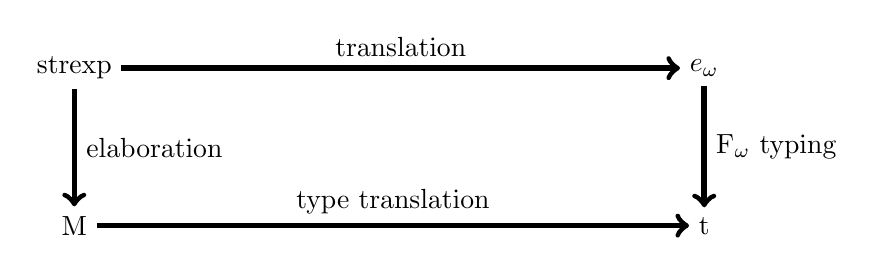
\begin{tikzpicture}[auto]
			\node (strexp) {strexp};
			\node[right of=strexp,node distance=8cm] (e) {$e_\omega$};
			\node[below of=strexp,node distance=2cm] (M) {M};
			\node[right of=M,node distance=8cm] (t) {t};
			
			\path[arr] (strexp) edge node {translation} (e);
			\path[arr] (e) edge node {F$_\omega$ typing} (t);
			\path[arr] (strexp) edge node {elaboration} (M);
			\path[arr] (M) edge node {type translation} (t);			
		\end{tikzpicture}
		% \begin{block}{Theorem}
		% 	If a structure expression $strexp$ elaborates to a full signature $M$ and $strexp$ translates to an F$_\omega$ expression $e_\omega$, then $e_\omega$ has F$_\omega$ type t and $M$ also translates to t.
		% \end{block} 
		\vspace{4mm}\\
		Proof: Induction on a strengthened version of the above. The proof depends on the correctness of type and value coercion, signature matching, and signature instantiation.
	\end{frame}
	
	\begin{frame}
		\frametitle{Main Ideas}
		\begin{enumerate}
			\itemsep=3mm
			\item Factoring module type information (full signature) into semantic signature and realization
			\item Entity calculus encodes functor actions
			\item Elaboration semantics in compilation and direct modes
			\item Coercive signature matching
		\end{enumerate}
	\end{frame}
	
	\begin{frame}
		\frametitle{Related Work: Syntactic Approach}
		\begin{itemize}
			\item CMU
		\begin{itemize}
			\item Harper-Lillibridge 1994, Harper-Stone 1997
			\item Dreyer-Crary-Harper 2003
			\item Harper-Pierce 2005
			\item Dreyer 2005, 2007
			\item Dreyer-Blume 2007
			\item Dreyer-Rossberg 2009
			\item Rossberg-Russo-Dreyer 2010
		\end{itemize}
			\item Leroy 1994, 1995, 1996, 2000
			\item Biswas 1995, Russo 2000
			\item Shao 1998, 1999
			\item Govereau 2005
			\item Montagu and R\'emy 2009
		\end{itemize}
	\end{frame}
		
	\begin{frame}
		\frametitle{Related Work: Semantic Approach}
		\begin{itemize}
			\itemsep=3mm
			\item MacQueen-Tofte 1994
			\item Cr\'egut and MacQueen 1994
			\item Shao 1998
			\item Kuan and MacQueen 2009
		\end{itemize}	
	\end{frame}
	
	\begin{frame}
		\frametitle{Future Work}
		\begin{enumerate}
			\itemsep=1cm
			\item Relationship to type classes
			\item Exceptions and modules
			\item Type inference and modules
		\end{enumerate}
	\end{frame}
		
	\begin{frame}
		\frametitle{Conclusion}
		\begin{itemize}
			\itemsep=4mm
			\item HO module semantics is analogous to $\beta$-reduction semantics
			\item Module types are and should be semantic
			\item One neither has to give up generative datatypes/functors nor true higher-order semantics for a practical semantics
		\end{itemize}
	\end{frame}
	
	\begin{frame}
		\frametitle{}
		{\Huge Thank You}
	\end{frame}
	
	\begin{frame}
		\frametitle{Syntactic Signature}
		Syntactic signatures are comprised of specs:
	\begin{columns}[t]
		\begin{column}{.7\textwidth}
			\begin{itemize}[<alert@+(1)>]
			\item[] \tikz[na] \node[coordinate] (n0) {}; type ($\alpha$, $\beta$) t 
			\item[] \tikz[na] \node[coordinate] (n1) {}; type s = int 
			\item[] \tikz[na] \node[coordinate] (n2) {}; structure M : sig type u end 
			\item[] \tikz[na] \node[coordinate] (n4) {}; val a : (M.u, s) t 
			\item[] \tikz[na] \node[coordinate] (n3) {}; functor F(X:T) : T 
			\end{itemize}
		\end{column}
		\begin{column}{.3\textwidth}
	\begin{itemize}
		\item[]<2-> \alert<2>{open tycon}
		\item[]<3-> \alert<3>{type definition}
		\item[]<4-> \alert<4>{structure}
		\item[]<5-> \alert<5>{value}
		\item[]<6-> \alert<6>{functor}
	\end{itemize}
		\end{column}
		\end{columns}

		\begin{tikzpicture}[overlay]
			\path[arr]<7> (n1) edge [bend left] (n0);
			\path[arr]<7> (n1) edge [bend right] (n2);

			\path[arr]<8> (n2) edge [bend left] (n0);
			\path[arr]<8> (n2) edge [bend left] (n1);

			\path[arr]<9> (n4) edge [bend left] (n0);
			\path[arr]<9> (n4) edge [bend left] (n1);
			\path[arr]<9> (n4) edge [bend left] (n2);

			\path[arr]<10> (n3) edge [bend left] (n0);
			\path[arr]<10> (n3) edge [bend left] (n1);
			\path[arr]<10> (n3) edge [bend left] (n2);
		\end{tikzpicture}
	\end{frame}
	
		\begin{frame}[fragile]
			\frametitle{Relativization}
	\begin{lstlisting}
	functor f() = 
	struct
	  datatype t = S of int
	  type u = t
	  val x : u = S 1
	end
	\end{lstlisting}
		
		\begin{block}{How to represent u in the signature?}
		\[ \lambda().\{ \rho_t = \newx(0), \rho_u = \rho_t \} \]
		\[ x : \rho_u \] 	
		\end{block}
		\end{frame}
		
	\begin{frame}
		\frametitle{Relativization}
		\begin{enumerate}
			\item Value and definitional tycon bindings must be relativized
			\item Look up first occurrence of atomic tycons in entity environment, the entity path mapping to that occurrence is the canonical entity path
			\item Replace atomic tycons with canonical entity path, entity paths which always point to the current instantiation given the current entity environment
		\end{enumerate}
		
	\end{frame}
		
		\begin{frame}[fragile]
			\frametitle{Signature Extraction}
			\begin{lstlisting}
			struct
			datatype t
			structure A = struct type u = t end
			functor F(X:sig type s end) = struct type v = X.s end
			end
			\end{lstlisting}
			
			\begin{eqnarray*}
			  & & t\mapsto (\rho_0, \tau^0) \\
			  & & A\mapsto \{u\mapsto (\rho_1, \rho_0)\} \\
			  & & F\mapsto (\rho_2, \Pi\rho_3:\{s\mapsto (\rho_4, 0)\}.\{v\mapsto \lambda().\rho_3\rho_4\})
			\end{eqnarray*}
		\end{frame}


		\begin{frame}
			\frametitle{Elaboration}
		  	\begin{itemize}
			    \item<1->    $\Gamma,\Upsilon,\Sigma\vdash sigexp \Rightarrow_{sig} \Sigma'$  signature elaboration
			    \item<2->   $\Gamma,\Upsilon,\Sigma\vdash fsgexp \Rightarrow_{fsg} \Sigma^f$  functor signature elaboration
			    \item<3-> $\Upsilon^{clo},\Upsilon^{lcl}\vdash \Sigma \uparrow \Upsilon^{lcl}$  signature instantiation
			    \item<4-> $\Upsilon\vdash\Gamma\hookrightarrow \Sigma$ signature extraction
			    \item<5-> $\Upsilon\vdash(M,\varphi):\Sigma\Rightarrow_{match} (M_c,\varphi_c)$  signature matching
			    \item<6-> $\Upsilon\vdash F \preceq \Sigma^f \Rightarrow_{fsgmtch} (\psi_c, \theta_c)$ functor signature matching
			    \item<7-> $\Gamma,\Upsilon\vdash d^m \Rightarrow_{decl} (\eta,\Gamma',\Upsilon')$  module declaration elaboration
			    \item<8-> $\Gamma,\Upsilon\vdash strexp \Rightarrow_{str} (M, \varphi)$  structure expression elaboration
			\end{itemize}
			
		\end{frame}
\end{document}